\section{Experimental Results}
We perform our experiments on the Dell T620 workstation with two 2.90GHz 8-cores 16-thread CPUs and 64 GB memory. We use the hostspot \cite{Huang:TVLSI'06} software to get the thermal stucuture of the microprocessors, and the number of the cores ranges from $9$ to $100$, and the distribution ranges from $3\times 3$ to $10 \times 10$. The size of the chip is $9mm\times 9mm \times 0.15mm$. Wattch \cite{Brooks:ISCA'00} is employed to get the power and instruction information with SPEC \cite{Henning:IEEEC'00} benchmarks. The ambient temperature is 20 $^\circ C$.

\begin{figure*}
\centering
  \subfigure[Result 1]
  {
    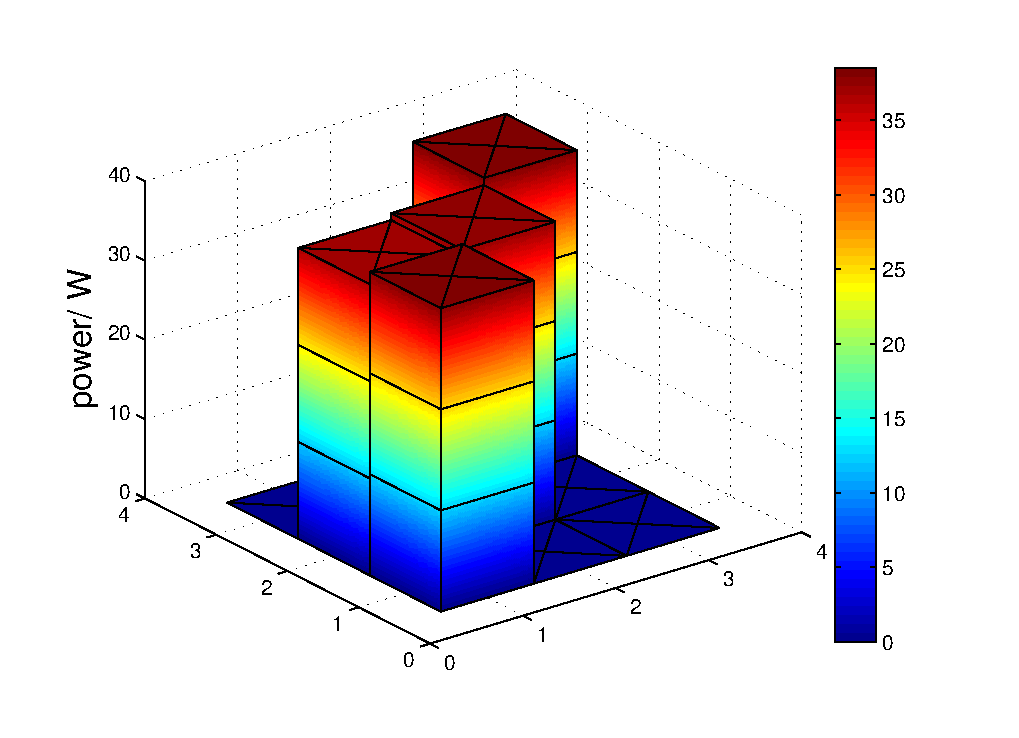
\includegraphics[width=0.4\textwidth]{fig/dis9_4_1.eps}
  }
 \subfigure[Result 2]
  {
    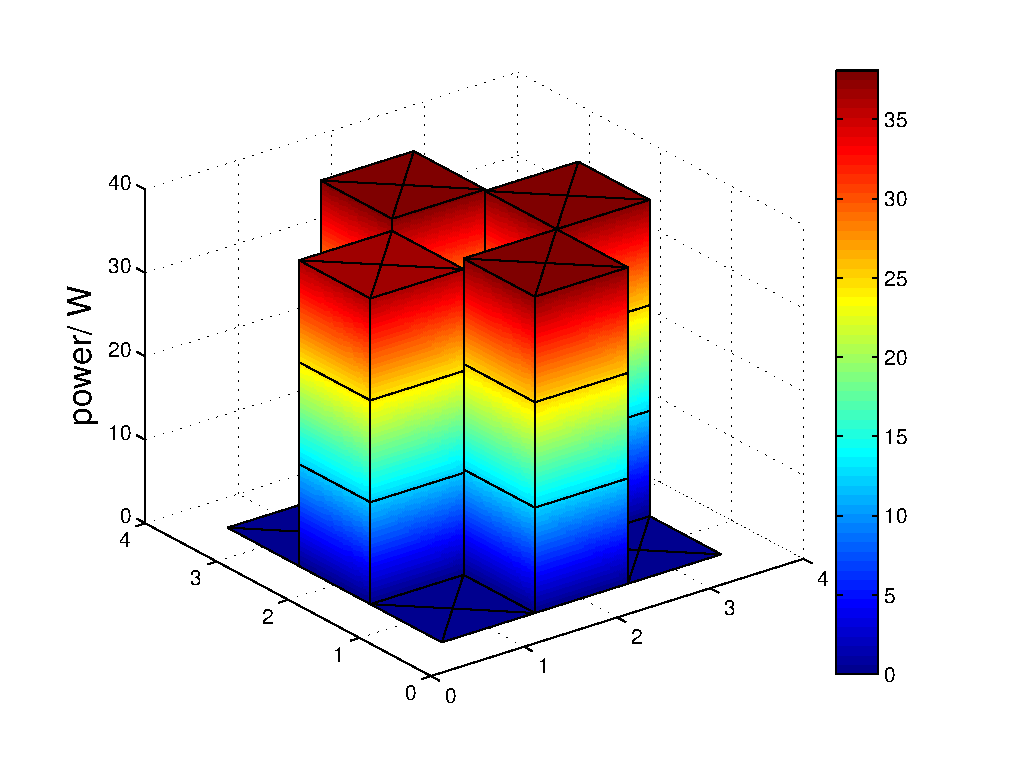
\includegraphics[width=0.4\textwidth]{fig/dis9_4_2.eps}
  }
\caption{Budgeting results of the active cores of the $3\times 3$ microprocessor with $4$ cores active at two time steps}\label{bud}
\end{figure*}

\begin{figure*}
  \centering
    \subfigure[Free run ]
  {
    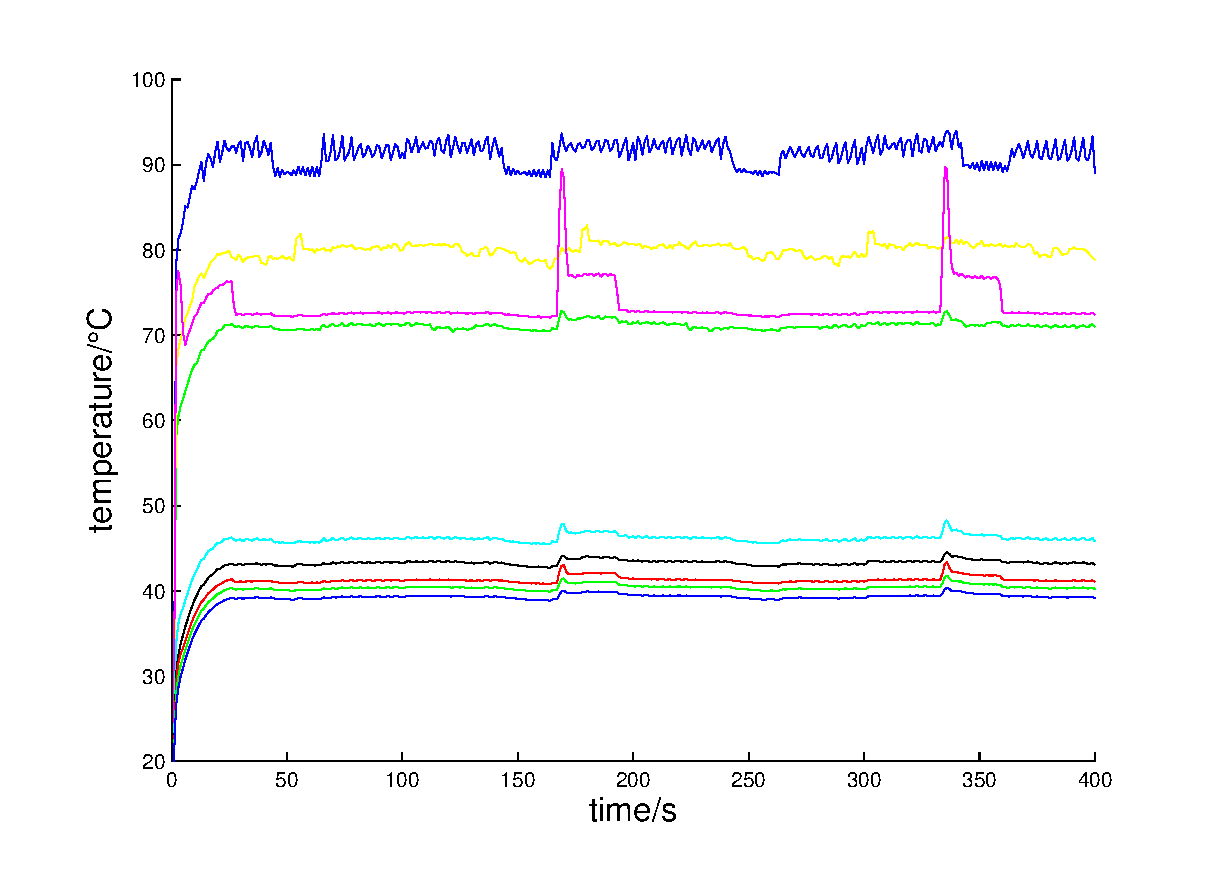
\includegraphics[width=0.4\textwidth]{fig/m9n4}
  }
    \subfigure[Using the new method]
  {
    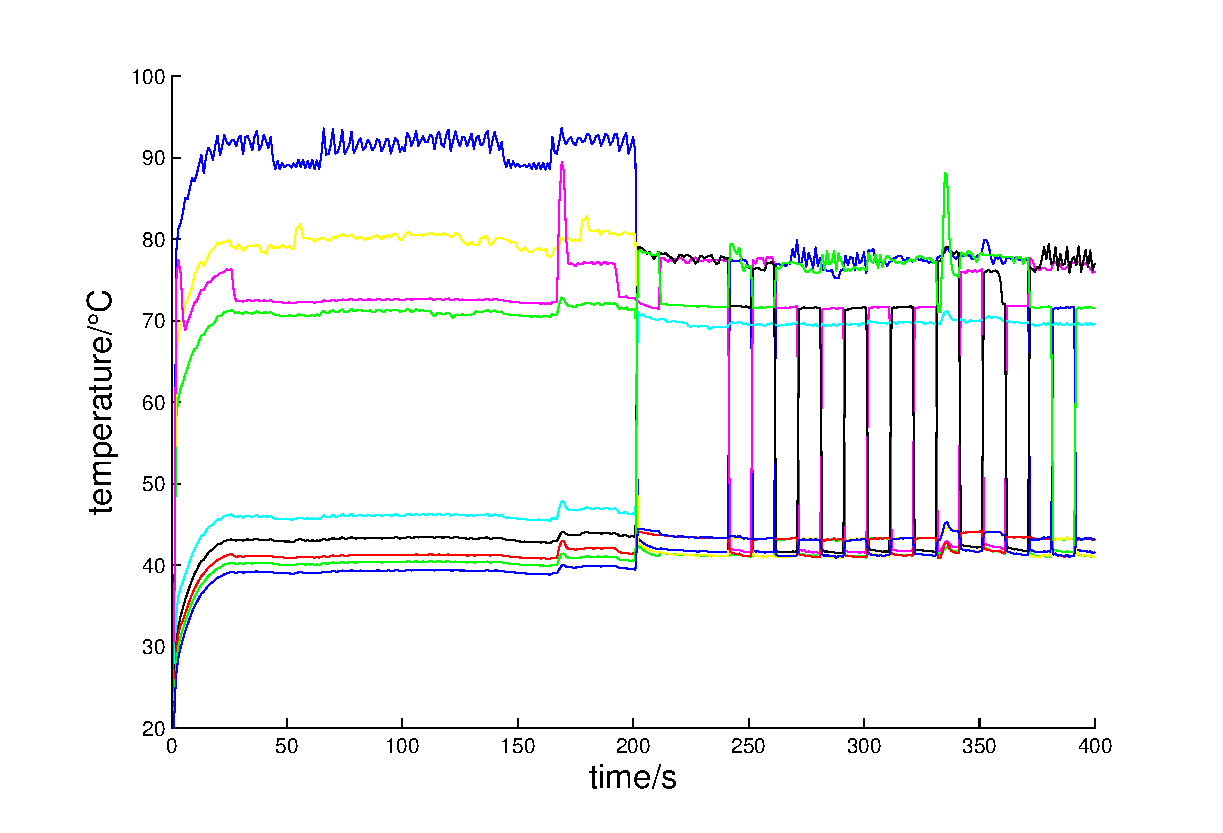
\includegraphics[width=0.4\textwidth]{fig/hungarym9n4t79j1}
  }
 \caption{Transient temperature of the $3\times 3$ microprocessor with $4$ cores active: Free run and the new method}\label{t_b}
\end{figure*}
\begin{figure*}
\centering
  \subfigure[Free run]
  {
    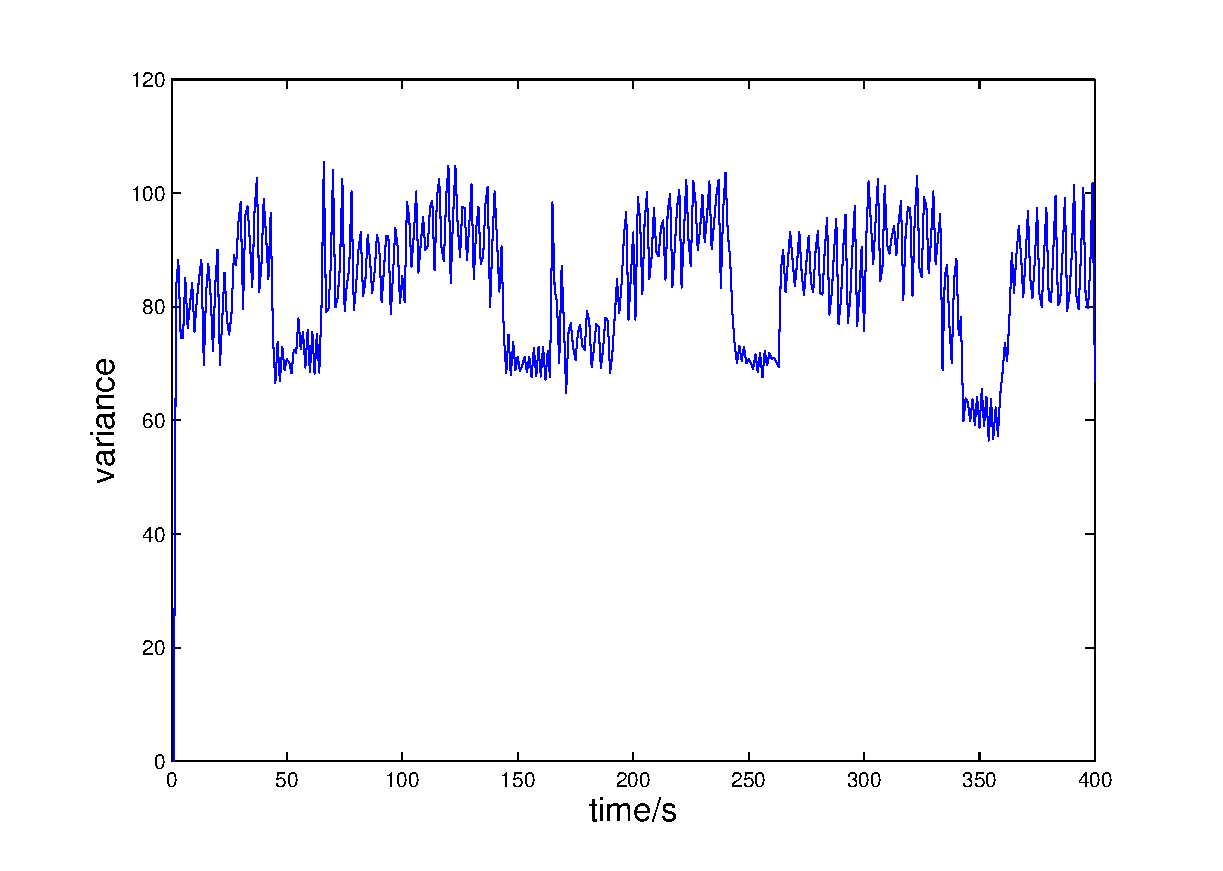
\includegraphics[width=0.4\textwidth]{fig/m9n4var}
  }
 \subfigure[The new method]
  {
    \includegraphics[width=0.4\textwidth]{fig/hungraym9n4varjunwen1}
  }
\caption{Transient variances of the active cores of the $3\times 3$ microprocessor with $4$ cores active: Free run and the new method}\label{var}
\end{figure*}
We take a $3\times 3$ cores microprocessor for example.

Fig. \ref{bud} shows the results of the new budgeting method at two different time steps. In Fig. \ref{bud}, the power of the active cores are presented and positions of the active cores are seperated. The result of the budgeting method can guides us to perform the optimal thermal management. 
In Fig.\ref{t_b}, we shows the transient temperature of free run without any thermal management and the one using the new method. And we set the target temperature to be $80^ \circ C $, and in Fig.\ref{t_b}(b), we use the new power budegting method and matching method after $200 s$. And the nearly vertical line means task migration which exchanges the power of different cores. Because we think that frequenctly performing task migration is harmful to the performance, we set the time step of $10s$ to use the power budgeting method and the matching method. The result is that at some points the temperature of the certain cores go beyond the target temperature. However, we can see that almost all the temperatures after $200 s$ are below the target temperature. So we suppose that this situation occupies little fraction of the whole time and will not cause much loss of the performance. And we can also see that the maximum temperature of the active cores are closely enough to the target temperature except for the very small extrem situations


From Fig.\ref{var}, we can see that after $200 s$, the variance of active cores' temperatures are significantly lower than the first $200 s$ and the free run one. The variance of the active cores show the difference of the temperature of the active cores, and lower variance means the active cores stay in the same working thermal environment which is useful for enhancing the lifetime of the chip. In table\ref{tab:time}, we show the $MIPS$ (Million instrucions per second) when $20\%$,$40\%$,$60\%$ of whole cores are active. And we use $j$ to represent the number of active cores. And we compared the result with DVFS. $MIPS_n$ refers to our new method, while $MIPS_d$ refers to DVFS. We can see that our new method is always better than DVFS, thus microprocessors can get better performance. 

  \begin{table*}[tbph]
%\tabcolsep=1pt
 \centering
 \caption{INSTRUCTIONS PER SECOND WITH DIFFERENT CONFUGURATIONS }~\label{tab:time} 
 \begin{tabular}{|c|c|c|c|c|c|c|c|c|c|}
 \hline
 \hline
        &   & \multicolumn{2}{|c|}{ $MIPS$} &  & \multicolumn{2}{|c|}{$MIPS$} & & \multicolumn{2}{|c|}{$MIPS$}\\
Configuration	& $j$ & $ MIPS_n$ & $MIPS_d$ & $j$ & $MIPS_n$ & $MIPS_d$ &  $j$ &$ MIPS_n$ & $MIPS_k$ \\ 
 \hline 
 \hline
 $3 \times 3$ & 2 & 174.72 & 146.11 & 4 & 323.26 & 287.40 & 6 & 415.12 &374.99 \\
 $4 \times 4$ & 3 & 130.89 & 115.05 & 6 & 234.40 & 211.05 & 9 & 408.32 &371.91 \\
 $5 \times 5$ & 5 & 108.32 & 98.28 & 10 &215.26 & 193.39  & 15 & 328.04 &297.81 \\
 $6 \times 6$ & 7 & 90.23 & 82.99 & 14 &   186.51& 168.88  & 22 & 290.38 &263.77 \\
 $7 \times 7$ & 10 & 90.97 & 80.81 & 20 & 174.53 & 157.26 & 30 & 265.40 & 242.23 \\
 $8 \times 8$ & 13 & 76.39 & 68.36 & 26 & 174.53 & 157.26 & 38 & 233.30 &213.45 \\
 $9 \times 9$ & 16 & 71.04 & 64.17 & 32 & 138.72 & 125.33 & 49 & 216.14 &194.26 \\
 $10 \times 10$ & 20 & 65.15 & 58.53 & 40 & 136.03 & 123.52 & 60 & 204.49 &186.11 \\
 \hline
 \hline
 \end{tabular}
 \end{table*}


